%!TEX root = ..\main.tex
\section{Model}
\label{sec:model}

\begin{figure*}[t]
\centering
	
\includegraphics[width=0.9\textwidth]{Images/fullSystemPicture}
	\captionsetup{justification=centering, width=0.9\textwidth}
	\caption{Snapshot for density $\rho = 0.95$ and $k_BT = 1.5$. Arrows represent the dipole moment of the particle. Obtained by means of Langevin dynamics simulation. The simulation was allowed to equilibrate for time $t = 100$ with fluid medium viscosity $\eta = 1$ and particle mass $m = 1$.}
	\label{fig:fullSystemPicture}
\end{figure*}

We consider colloidal particles with a permanent dipole moment $\mu \hat{m}$, where $\hat{m}$ is a unitary vector with the direction of the dipole moment. While considering a three-dimensional system, we constrain particle translational motion to a one-dimensional line, i.e. particles are confined to the $z$ axis. However, particles can explore the full three-dimensional orientation space. A snapshot of the system is shown in the \figref{fig:fullSystemPicture}.

The particle-particle interaction is described as the superposition of two contributions: a dipole-dipole interaction and a short-range repulsion.

The energy of dipole-dipole interaction for any pair (i, j) of particles is given by

\begin{equation}
\label{eq:dipole_dipole_interaction}
U^{dip}_{ij} =
	- \frac{\mu_i \mu_j}{\Delta r^3}[
		3 (\hat{m}_i \cdot \hat{r}_{ij})(\hat{m}_j \cdot \hat{r}_{ij})
		- (\hat{m}_i \cdot \hat{m}_j)
	]
\end{equation}
where $\mu_i \hat{m}_i$ and $\mu_j \hat{m}_j$ are dipole moments of interacting particles, $\boldsymbol{r}_{ij}$ is the direction vector which connects particle centers, and $\Delta r$ is the absolute value of the distance between particle centers.

By constraining particles to a 1D tube we effectively enforce $\boldsymbol{r}_{ij}$ to be co-aligned with $z$ axis. Assuming that all particles have the same dipole moment $\mu_i = \mu_j = \mu$, and defining $\mu = 1$ \eqref{eq:dipole_dipole_interaction} can be simplified as:

\begin{equation}
\label{eq:dipole_dipole_1D}
E_{ij}^{dip} = - \frac{1}{\Delta z^3} [3 \cos \theta_i \cos \theta_j - (\hat{m}_i \cdot \hat{m}_j)]
\end{equation}
where $\theta_i$ and $\theta_j$ are the angles between $z$ axis and dipole moments of the first and second particle, respectively, and $\Delta z = |z_j - z_i|$, where $z_i$ and $z_j$ are particle positions along the $z$ axis.

The repulsive part is described by Yukawa potential
\begin{equation}
\label{eq:yukawa_interaction}
E_{ij}^{rep} = \frac{A \exp(-k \Delta z)}{\Delta z},
\end{equation}
where $A$ and $k^{-1}$ are the strength and range of interaction. 

In this work we define thermal energy $\epsilon$ as fraction of dipole-dipole interaction potential, i.e. $\epsilon = k_BT \mu^2$, and maintaining the ration between $\mu$ and $A$ as constant. Since $\mu = 1$, we will use $k_BT$ to denote thermal energy. \textcolor{red}{I mean, it's the same value, but different units, right}

\figref{fig:interaction_energy} shows some examples of $E_{ij}$ for different parameters.

\begin{figure}[p]
\centering
	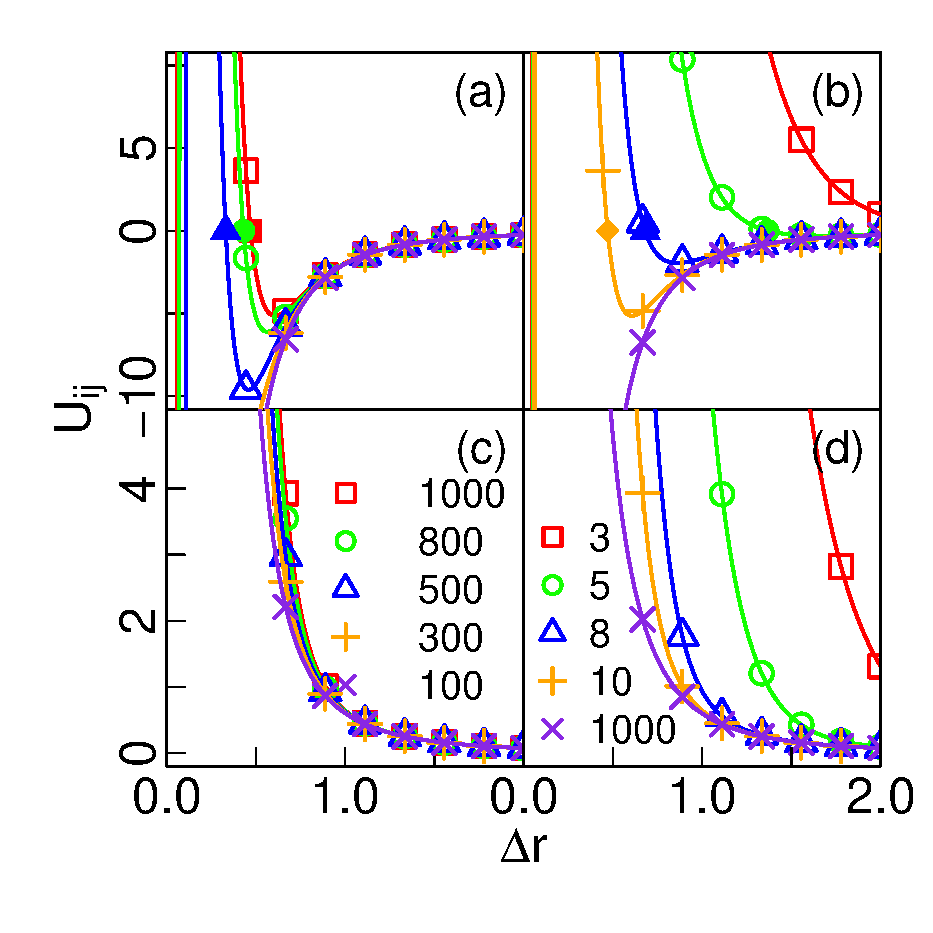
\includegraphics[width=0.9\textwidth]{Images/particle_interaction_potential}
\captionsetup{justification=centering, width=0.9\textwidth}
\caption{Potential energy as function of the interparticle distance when the dipoles are aligned (top) and perpendicular (bottom) orientation of the particles dipole moments. Left plots the interparticle distance when the dipoles are for $k = 10$, and right the right ones for $A = 1000$.}
\label{fig:interaction_energy}
\end{figure}

When the dipole moments are perpendicular to each other, the interaction is purely repulsive for any given $A$ and $k$.

However, as we can see on the Figs.~\ref{fig:interaction_energy}(a)~and~(b), for co-aligned configurations for significantly low values of $A$ and high values of $k$, the interaction is purely attractive. We will not consider those cases, as the system will be unstable and all particles will coalesce in one point. In this work, to reduce the number of free-parameters we fix $A = 1000 \mu$ and $k = 10$. \textcolor{red}{The $k$ is inverse distance, right?}
